\chapter{Spørgsmål}

\section{Spørgsmål 1}
\textit{Hvad er PRINCE2´s definitionen på et projekt?}

En midlertidig organisation til formål at levere ét eller flere produkter i henhold til en \nameref{sec:business_case}.

\section{Spørgsmål 2}
\textit{Hvad karakteriserer et projekt i forhold til daglig drift?}

Projekter eksisterer midlertidigt og kan involvere et bredt spektrum af organisationsmedlemmer, hvor daglig drift typisk involverer de samme medlemmer og ledelse i en mere permanent form.


\section{Spørgsmål 3}
\textit{Overvej hvorfor det er centralt for PRINCE2, at projekter laves af en midlertidig projektorganisation som udnævnes til projektet, i stedet for blot at lade "line management" (linjeledelsen) lave projekterne}

En midlertidigt projektstruktur tillader bedre tværorganisatorisk sammearbejde og gør det letter at sammensætte en organisation, der passer til den business case, der er relevant for projektet.

\section{Spørgsmål 4}
\textit{Hvilke 6 præstationsmål(Performance Targets) har PRINCE2 fokus på?}

\begin{itemize}
    \item Tidsomkostninger
    \item Resourceomkostninger
    \item Kvalitet
    \item Scope
    \item Udbytte
    \item Risks
\end{itemize}

\section{Spørgsmål 5}
\textit{Figur 11.2 PRINCE2 manualen er en oversigt over PRINCE2´s procesmodel. Indsæt et screendump af den her.}

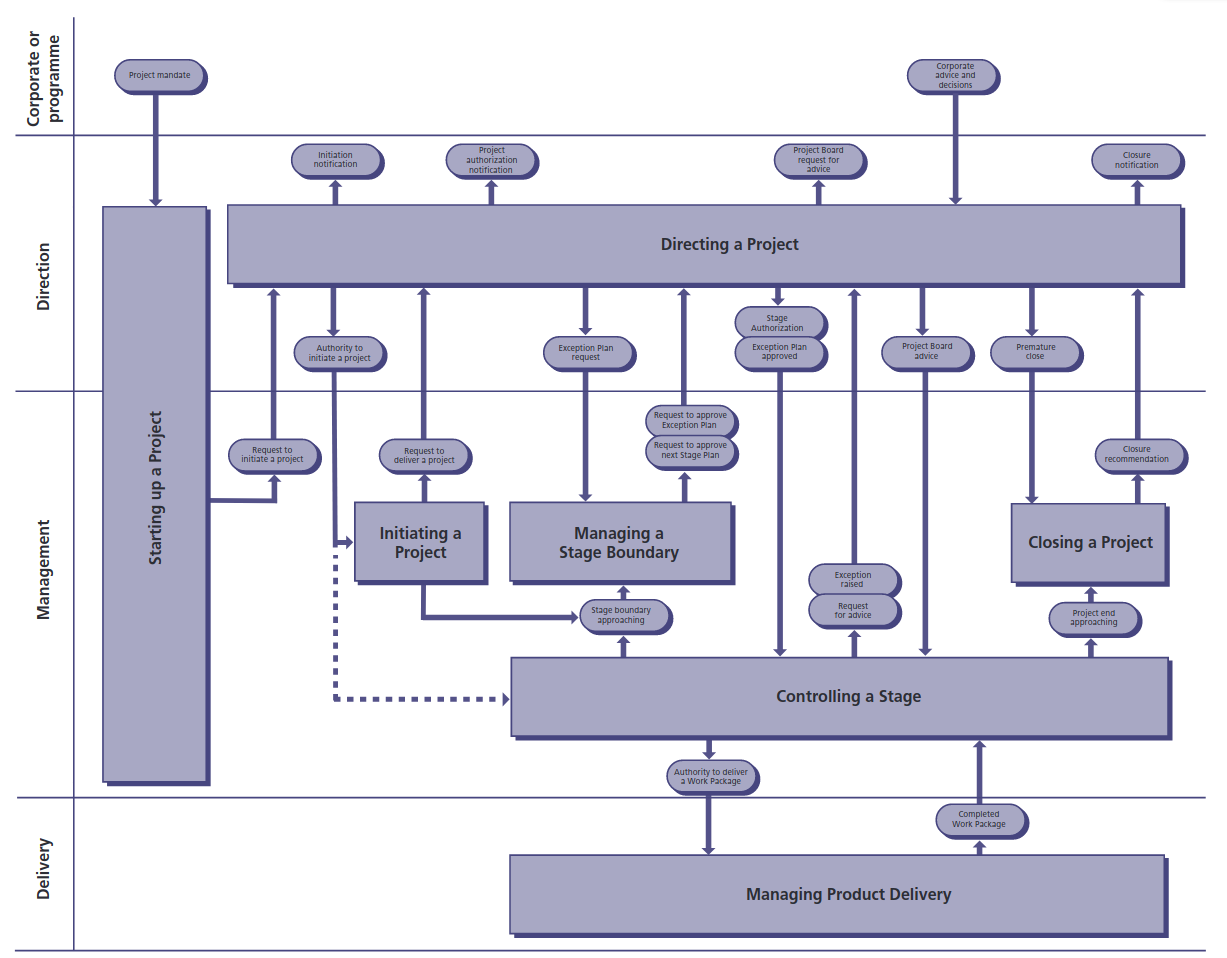
\includegraphics{prince2.includes/figure112.png}

\section{Spørgsmål 6}
\textit{Find ”Project Mandate”(projektkommissoriet) på PRINCE2´s procesmodel på figur 11.2}
\section{Spørgsmål 7}
\textit{Lav en kort sammenfatning over formålet med projektkommissoriet(Project Mandate) (1- 2 sætninger)}
\section{Spørgsmål 8}
\textit{Hvilke oplysninger bør findes i projektkommissoriet(Project Mandate)?}
\section{Spørgsmål 9}
\textit{Skal projektets forventede udbytte(Benefits) altid kvantificeres?}
\section{Spørgsmål 10}
\textit{Skal projektets udbytter(Benefits) altid udtrykkes som økonomiske fordele?}
\section{Spørgsmål 11}
\textit{Hvem er operationelt ansvarlig for at det udbytte(Benefit) der står i Business Casen også bliver realiseret?}
\section{Spørgsmål 12}
\textit{Hvornår udarbejdes Plan for Udbyttereview(Benefits Review Plan)?}
\section{Spørgsmål 13}
\textit{Lav en kort beskrivelse af formålet med at have en projektorganisation (1-5 linjer)}
\section{Spørgsmål 14}
\textit{Er en projektorganisation midlertidig eller fast?}
\section{Spørgsmål 15}
\textit{Hvor mange niveauer indgår i en PRINCE2 projektorganisation? Hvilke?}
\section{Spørgsmål 16}
\textit{Hvilke tre interesser indgår i et projekt, og hvilken rolle har fokus på at varetage forretningens interesse?}
\section{Spørgsmål 17}
\textit{Hvilken rolle kan det være vanskeligt at fastsætte før projektfremgangsmåden er fastlagt?}
\section{Spørgsmål 18}
\textit{Hvor mange personer er der mindst involveret i et PRINCE2 projekt?}
\section{Spørgsmål 19}
\textit{Forestil dig, at du arbejder i en kommune skal have nye PC’ere på deres skoler. Du er blevet bedt om at være Projektleder, og møder for første gang Styregruppen(Project Board), som omfatter 23 personer. Hvad vil du anbefale Styregruppen(Project Board)?}
\section{Spørgsmål 20}
\textit{Hvad bruges Kvalitetsregisteret(Quality Register) til under Planlægningen af den næste fase?}
\section{Spørgsmål 21}
\textit{I hvilken proces udarbejdes projektets Slutproduktbeskrivelse(Project Product Description)?}
\section{Spørgsmål 22}
\textit{Hvornår udarbejdes Produktbeskrivelserne(Product Descriptions)?}
\section{Spørgsmål 23}
\textit{Hvor er Kvalitetstolerancerne(Quality Tolerance) beskrevet, i hvilken sammenhæng?}
\section{Spørgsmål 24}
\textit{Hvor er Kvalitetskriterierne(Quality Criteria) beskrevet, i hvilken sammenhæng?}
\section{Spørgsmål 25}
\textit{Hvad anvender man Slutproduktbeskrivelsen(Project Product Description) til?}
\section{Spørgsmål 26}
\textit{Kan man ændre i Slutproduktbeskrivelsen(Project Product Description), efter Start af et Projekt(Starting a Project) processen og i givet fald, hvem kan godkende ændringer?}
\section{Spørgsmål 27}
\textit{Hvorfor skal projektfremgangsmåden(Project Approach) bestemmes allerede i Start af et Projekt(Starting up a Project)? Kan man ikke vente med at definere fremgangsmåden, når man laver Projektplanen(Project plan) i Initiering af et Projekt(Initiating a Project) processen?}
\section{Spørgsmål 28}
\textit{Hvor er detaljerne omkring datoer, omkostninger og milepæle beskrevet?}
\section{Spørgsmål 29}
\textit{Hvorfor er det vigtigt at have taget stilling til Risikostyringsstrategien(Risk Management Strategy) for et projekt?}
\section{Spørgsmål 30}
\textit{Hvad har man i virkeligheden besluttet, hvis man ikke vil anvende ressourcer til risikostyring(Risk Management)?}
\section{Spørgsmål 31}
\textit{Hvad skal Teamlederen(Team Manager) gøre så snart han/hun bliver bekendt med at de planlagte produkter(Work Package) ikke kan afleveres inden for tolerancerne(Tolerances)?}
\section{Spørgsmål 32}
\textit{Hvor er detaljerne omkring disse tolerancer(Tolerances) beskrevet?}
\section{Spørgsmål 33}
\textit{Hvad skal Teamlederen(Team Manager) gøre så snart han/hun bliver bekendt med at de planlagte produkter(Work Package) ikke kan leveres i henhold til forventningerne(Expectations)?}
\section{Spørgsmål 34}
\textit{Hvad er PRINCE2 termen for disse forventninger(Expectations) og hvor er de beskrevet?}
\section{Spørgsmål 35}
\textit{Hvad er de 4 karakteristika (characteristics) som alle medlemmer af Styregruppen(Project Board) bør besidde?}
\section{Spørgsmål 36}
\textit{Vi hører ofte fra organisationer, at det hos dem er det projektlederen(Project Manager) der har det overordnede ansvar for projektet. Kan dette være en god idé, eller er det uhensigtsmæssigt? Begrund dit svar.}
\section{Spørgsmål 37}
\textit{Hvilke 3 registre oprettes i initieringsfasen(Initiation a Project)?}
\section{Spørgsmål 38}
\textit{Hvilket budget er tæt forbundet med konfigurationsstyring(Configuration Management)? Begrund dit svar.}
\section{Spørgsmål 39}
\textit{Hvilket ledelsesprodukt(Management Product) anvendes til at registrere gennemførte kvalitetsaktiviteter(Quality Activities)?}
\section{Spørgsmål 40}
\textit{Hvornår registreres planlagte kvalitetssikringsaktiviteter(Quality Assurance Activities)?}
\section{Spørgsmål 41}
\textit{Hvornår begynder Styregruppens(Project Board) arbejde i projektet: Før eller efter beslutningen om at godkende initiering? Begrund dit svar.}
\section{Spørgsmål 42}
\textit{Hvornår kan Styregruppen(Project Board) afslutte et projekt?}
\section{Spørgsmål 43}
\textit{Giv nogle begrundelse for, hvorfor en Styregruppe(Project Board) kan vælge at afslutte et projekt før tid.}
\section{Spørgsmål 44}
\textit{Hvad skal der ske, når et PRINCE2 projekt afsluttes, uanset om det afsluttes i utide eller i henhold til planen?}
\section{Spørgsmål 45}
\textit{På et møde i den virksomhed, som du arbejder i, diskuterer I at implementere PRINCE2 i afdelingen, men flere udtrykker bekymring over, at man får et stort og besværligt projektbureaukrati. Derfor bliver det besluttet at indføre en ”PRINCE light” version. Hvad er din kommentar til dette?}
\section{Spørgsmål 46}
\textit{Hvor i projektets dokumentation beskriver man, hvorledes PRINCE2 er tilpasset det pågældende projekt?}
